\section{Results}\label{results}

\noindent When collecting results from the model it is essential to be consistent with the parameters already chosen in Section \ref{parametertests}. For cases where two masses are of equal mass, they will be 50kg each, as in the tests. When the masses represent a child and adult, the masses will differ. The average weight of an 11 year old child was found to be 35.6 kg \cite{childweight}, with a maximum jumping height assumed to be 1.44m, the height of the child \cite{childweight} and a reasonable decision for the weight of a young adult was assumed to be 70 kg with a maximum jumping height of 1.8m, the corresponding height of the adult.
\\
\\
\noindent The model can be tested to produce a variety of results that will provide information about interaction between two people on a trampoline. Analysing what happens at different time-steps, explained in Section \ref{combine}, between when the two masses are in contact with the trampoline is achieved by dropping the masses at a range of different times. The maximum heights reached by the masses for this range are plotted. This is discussed in Section \ref{res1}.
\\
\\
\noindent Varying the distance between the two masses will also affect the maximum height reached. This is discussed in Section \ref{res2}

\subsection{3D Graph Analysis}\label{3d}
%%% 3d graphs. 
\noindent Figures \ref{fig:m1on3d}, \ref{fig:m2on3d} and \ref{fig:msameon3d} look at the maximum heights reached by a chosen mass given certain testing conditions. They provides information about the maximum height reached for the ranges of the initial conditions, time-step and distance between masses. The number of time-steps used is 250 to produce smooth results and the distances between masses ranges between 0.3m and 2.5m. These graphs offer a useful visualisation of the behaviour of the system.

%%% regardless of starting heights of either mass same shape happens. The graphs show that which ever mass hits the trampoline first is the one that is bounced higher. 




\begin{figure}[H]
	\centering
    \begin{subfigure}{0.45\textwidth}
		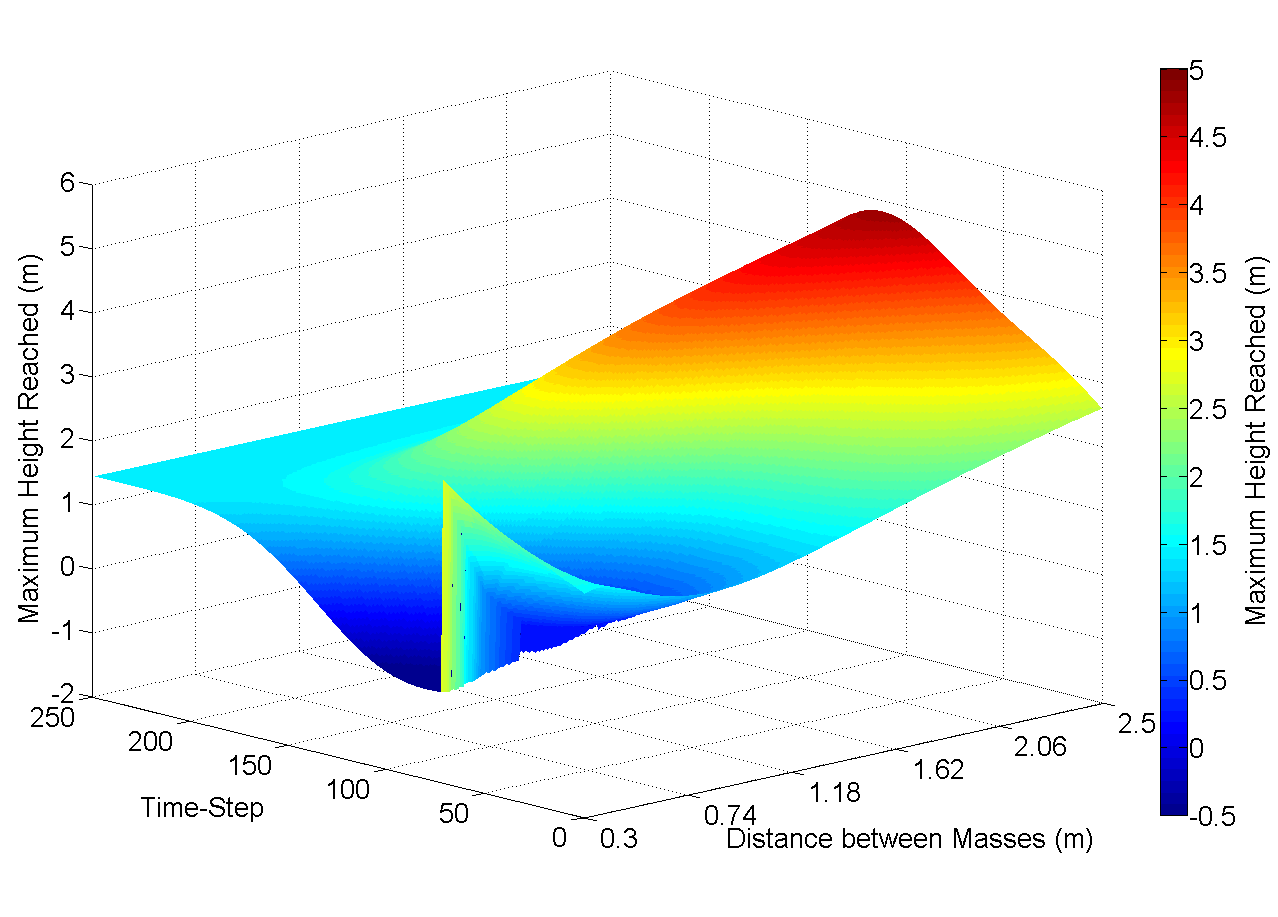
\includegraphics[width=3.1in, height=3.1in]{m1_on_tramp_different_masses_m1.png}
    	\caption{The maximum height of mass one.}\label{fig:m1m1}
    \end{subfigure}\hfill
	\begin{subfigure}{0.45\textwidth}
		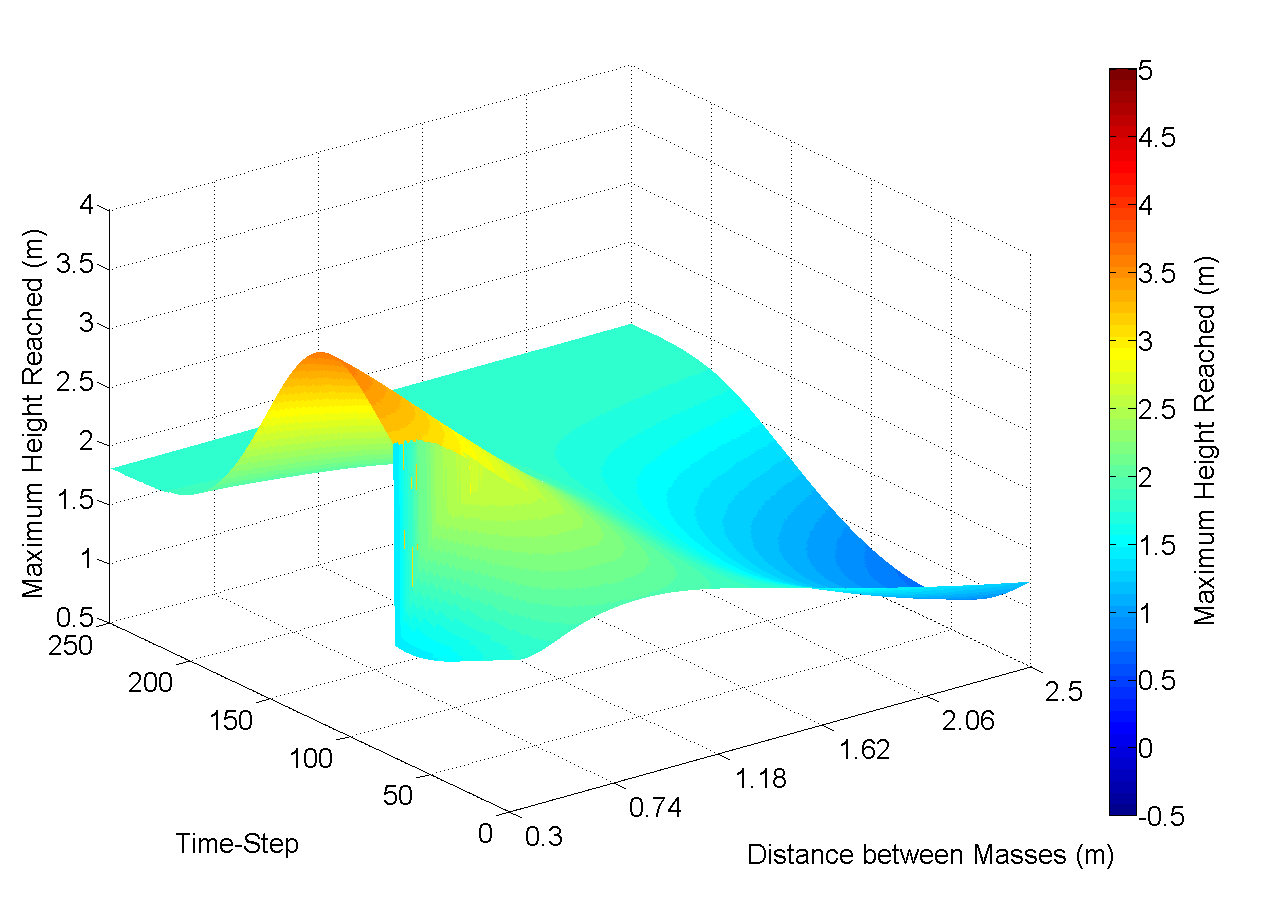
\includegraphics[width=3.1in, height=3.1in]{m1_on_tramp_different_masses_m2.png}
    	\caption{The maximum height of mass two.}\label{fig:m1m2}
    \end{subfigure}\hfill
    \caption{Graphs showing heights of mass one, 35.6kg, and mass two, 70kg, when mass one is dropped on trampoline first.}\label{fig:m1on3d}
\end{figure}

\begin{figure}[H]
	\centering
    \begin{subfigure}{0.45\textwidth}
		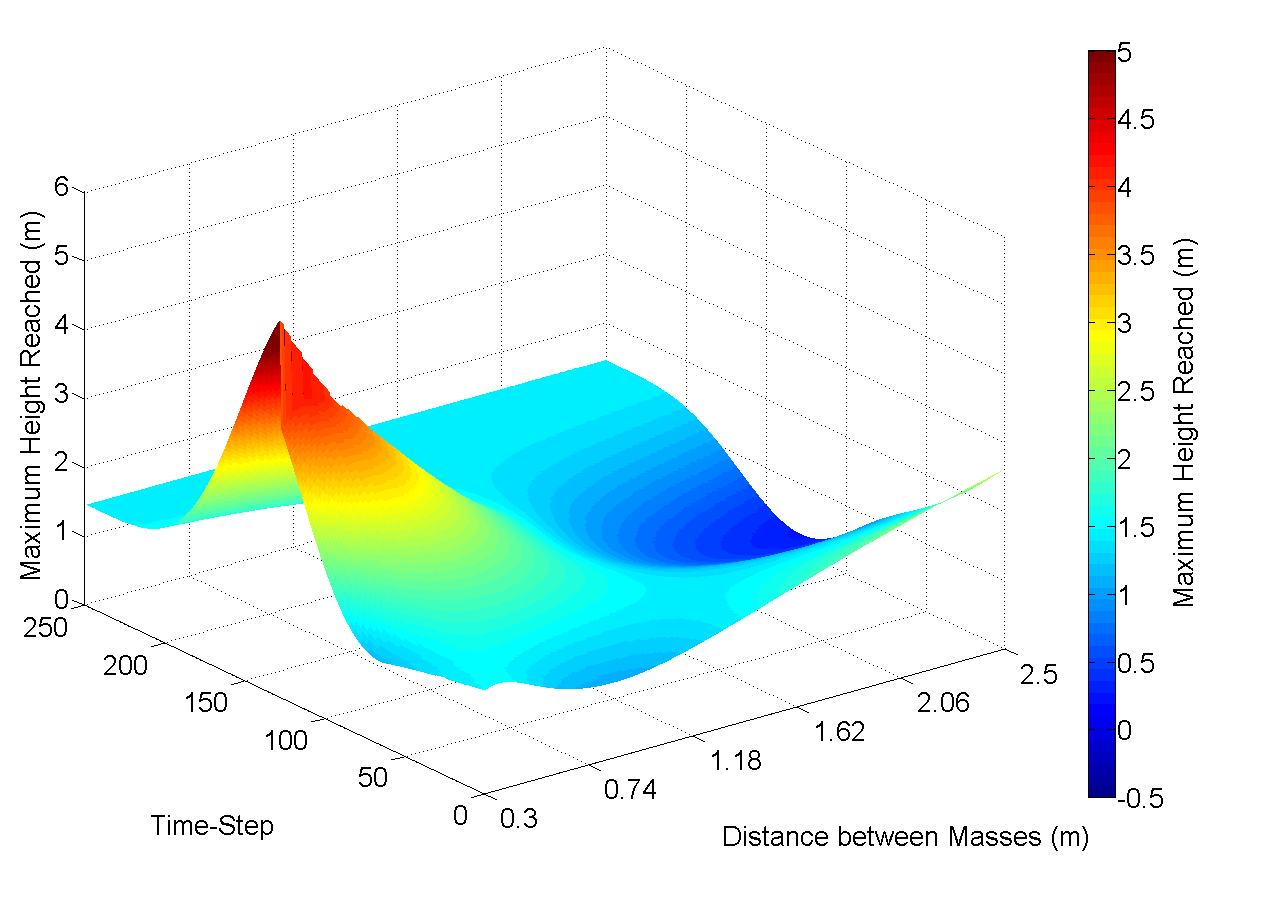
\includegraphics[width=3.1in, height=3.1in]{m2_on_tramp_different_masses_m1.png}
    	\caption{The maximum height of mass one.}\label{fig:m2m1}
    \end{subfigure}\hfill
	\begin{subfigure}{0.45\textwidth}
		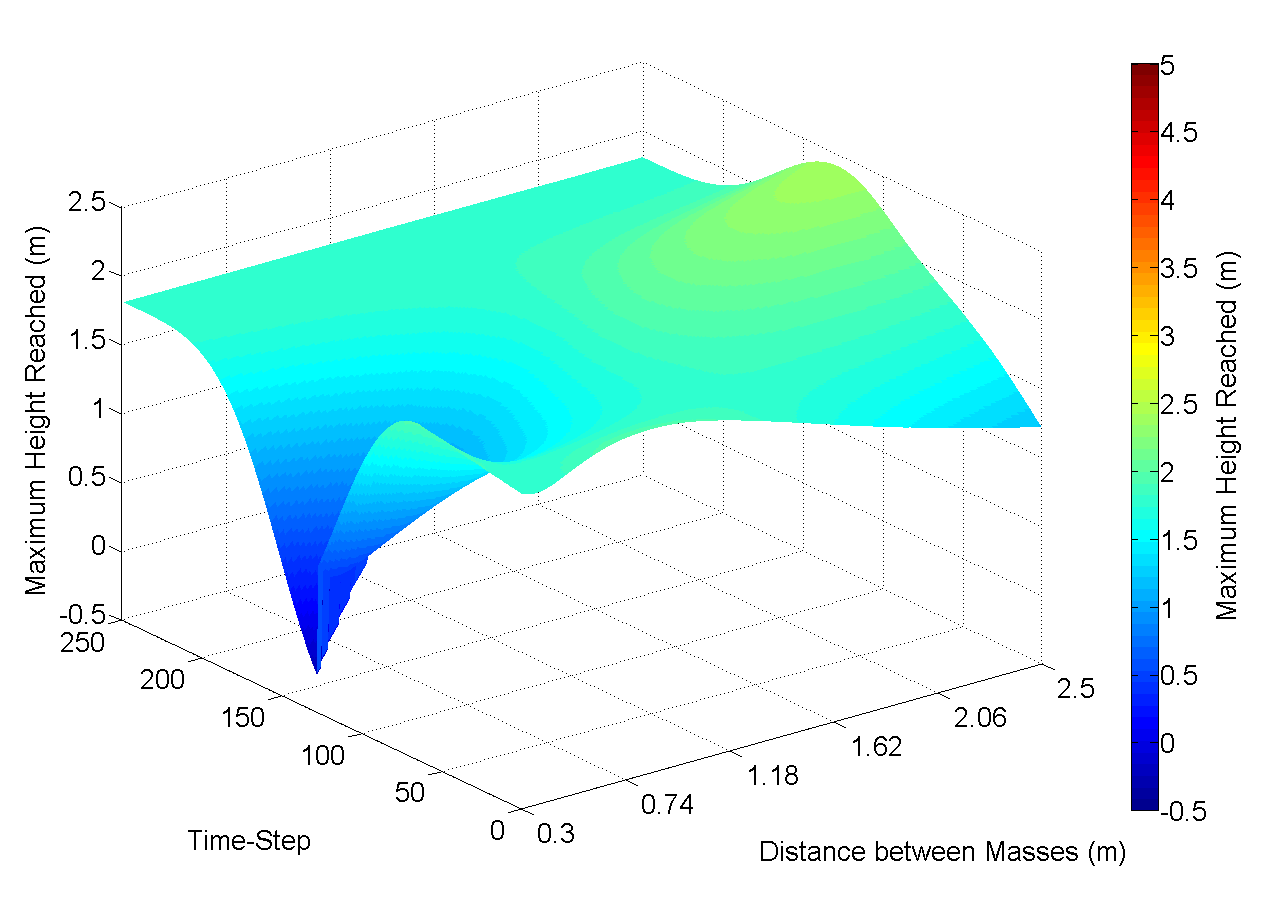
\includegraphics[width=3.1in, height=3.1in]{m2_on_tramp_different_masses_m2.png}
    	\caption{The maximum height of mass two.}\label{fig:m2m2}
    \end{subfigure}\hfill
    \caption{Graphs showing heights of mass one, 35.6kg, and mass two, 70kg, when mass two is dropped on trampoline first.}\label{fig:m2on3d}
\end{figure}

\begin{figure}[H]
	\centering
    \begin{subfigure}{0.45\textwidth}
		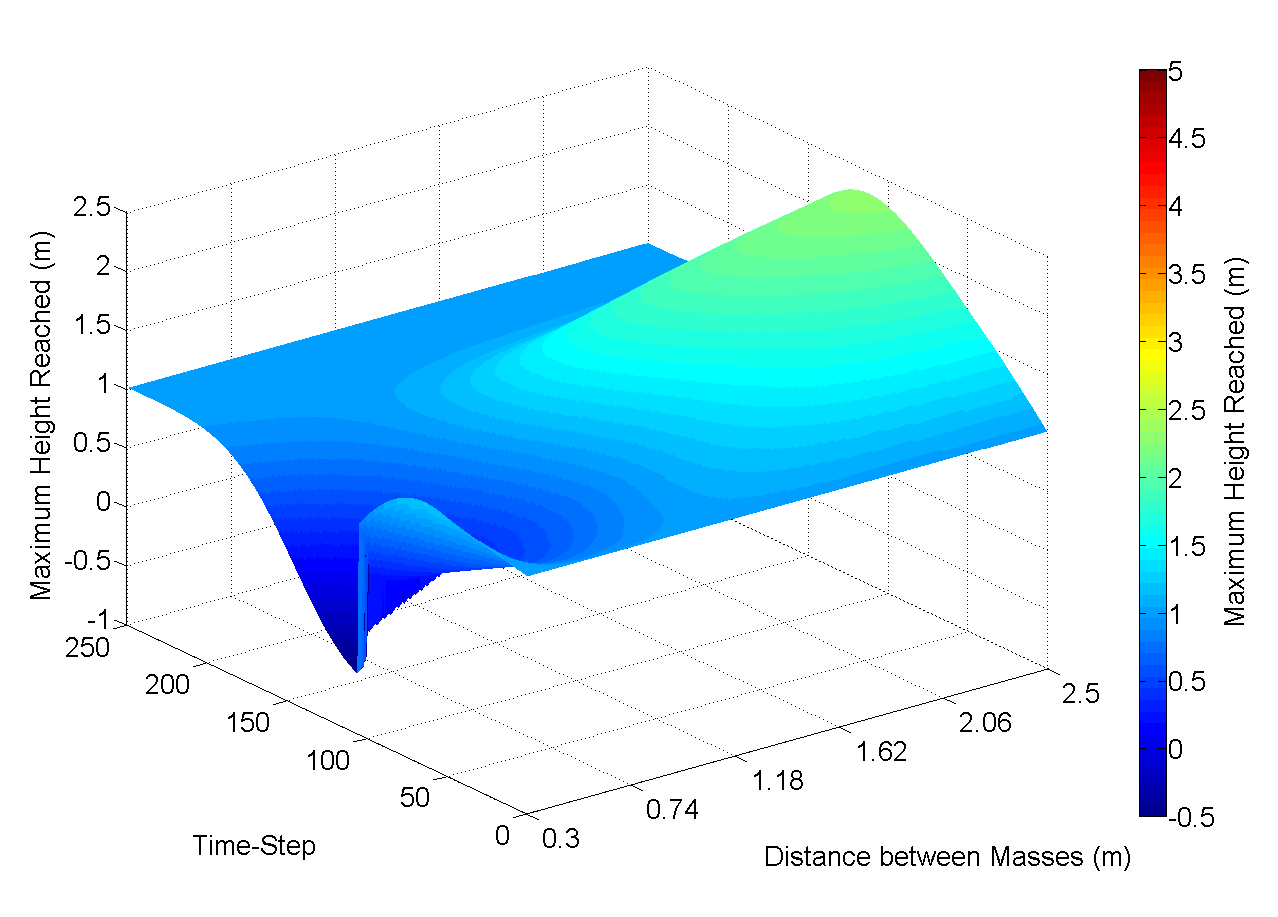
\includegraphics[width=3.1in, height=3.1in]{m1_on_tramp_same_masses_m1.png}
    	\caption{The maximum height of mass one.}\label{fig:m1samem1}
    \end{subfigure}\hfill
	\begin{subfigure}{0.45\textwidth}
		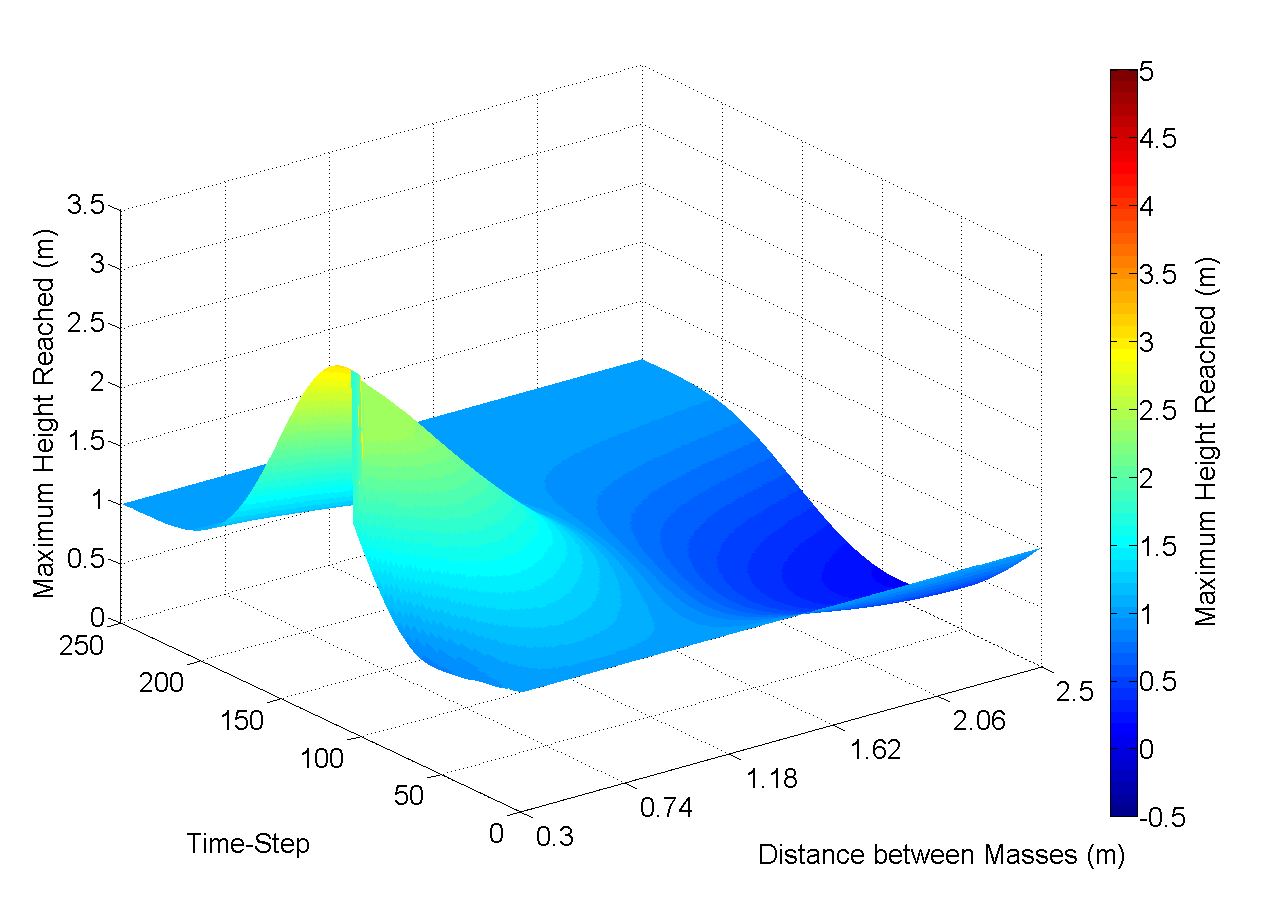
\includegraphics[width=3.1in, height=3.1in]{m1_on_tramp_same_masses_m2.png}
    	\caption{The maximum height of mass two.}\label{fig:m1samem2}
    \end{subfigure}\hfill
    \caption{Graphs showing heights of mass one and two when mass one is dropped on trampoline first and masses are both 50kg.}\label{fig:msameon3d}
\end{figure}




\subsection{Modelling Masses Dropped at Different Time-steps}\label{res1}

\noindent By studying how the masses interact with each other and the trampoline when they are said to bounce at similar or differing times will give some information about what circumstances it is safe for two people to use a trampoline at the same time is. By taking a 'slice' of the three dimensional graphs in Figures \ref{fig:m1on3d}, \ref{fig:m2on3d} and \ref{fig:msameon3d} above for a selected distance, taken to be constant for all tests for the sake of consistency, analysis into at how energy is transferred between masses dropped causing height variations for all time-steps. This distance was chosen to be 1.4 metres.% edit.
\\
\\
\begin{figure}[H]
	\centering
    \begin{subfigure}[t]{0.3\textwidth}
		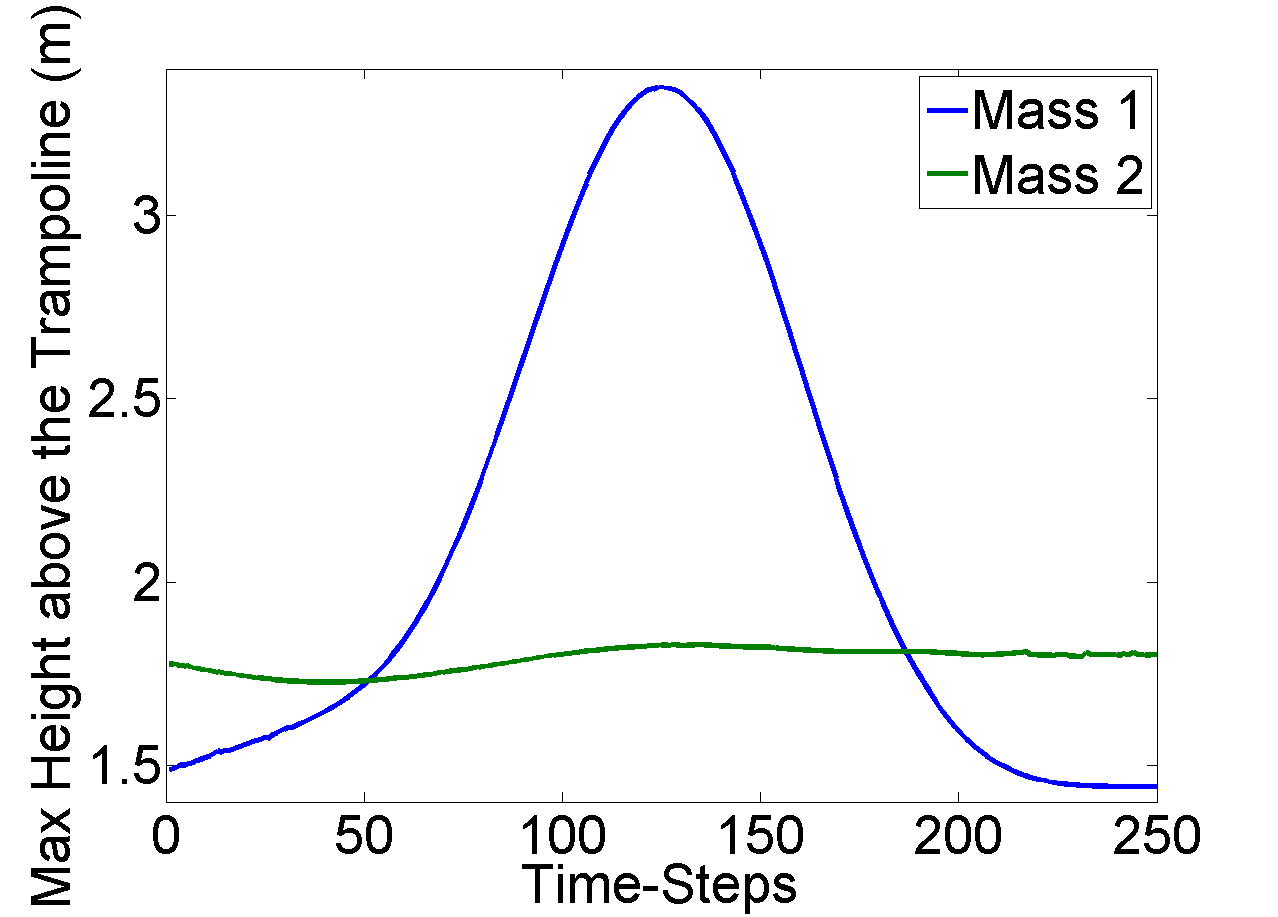
\includegraphics[width=\textwidth]{m1_on_tramp_different_masses_distance_14.png}
    	\caption{Maximum heights reached when $m_1$ and $m_2$ are different masses and $m_1$ starts on the trampoline.}\label{fig:m1_on_tramp_different_masses_distance_14}
    \end{subfigure}\hfill
	\begin{subfigure}[t]{0.3\textwidth}
		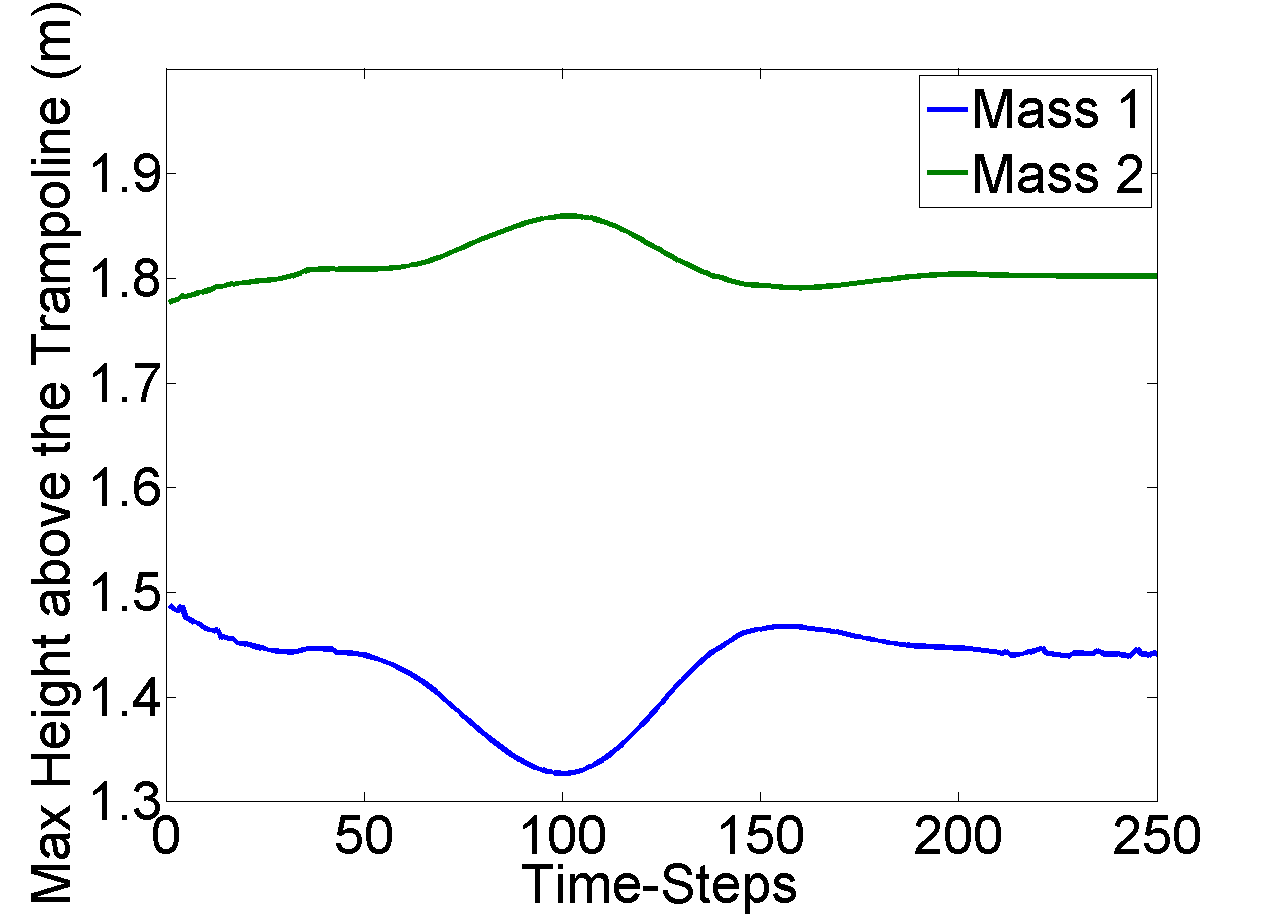
\includegraphics[width=\textwidth]{m2_on_tramp_different_masses_distance_14.png}
    	\caption{Maximum heights reached when $m_1$ and $m_2$ are different masses and $m_2$ starts on the trampoline.}\label{fig:m2_on_tramp_different_masses_distance_14}
    \end{subfigure}\hfill
    \begin{subfigure}[t]{0.3\textwidth}
		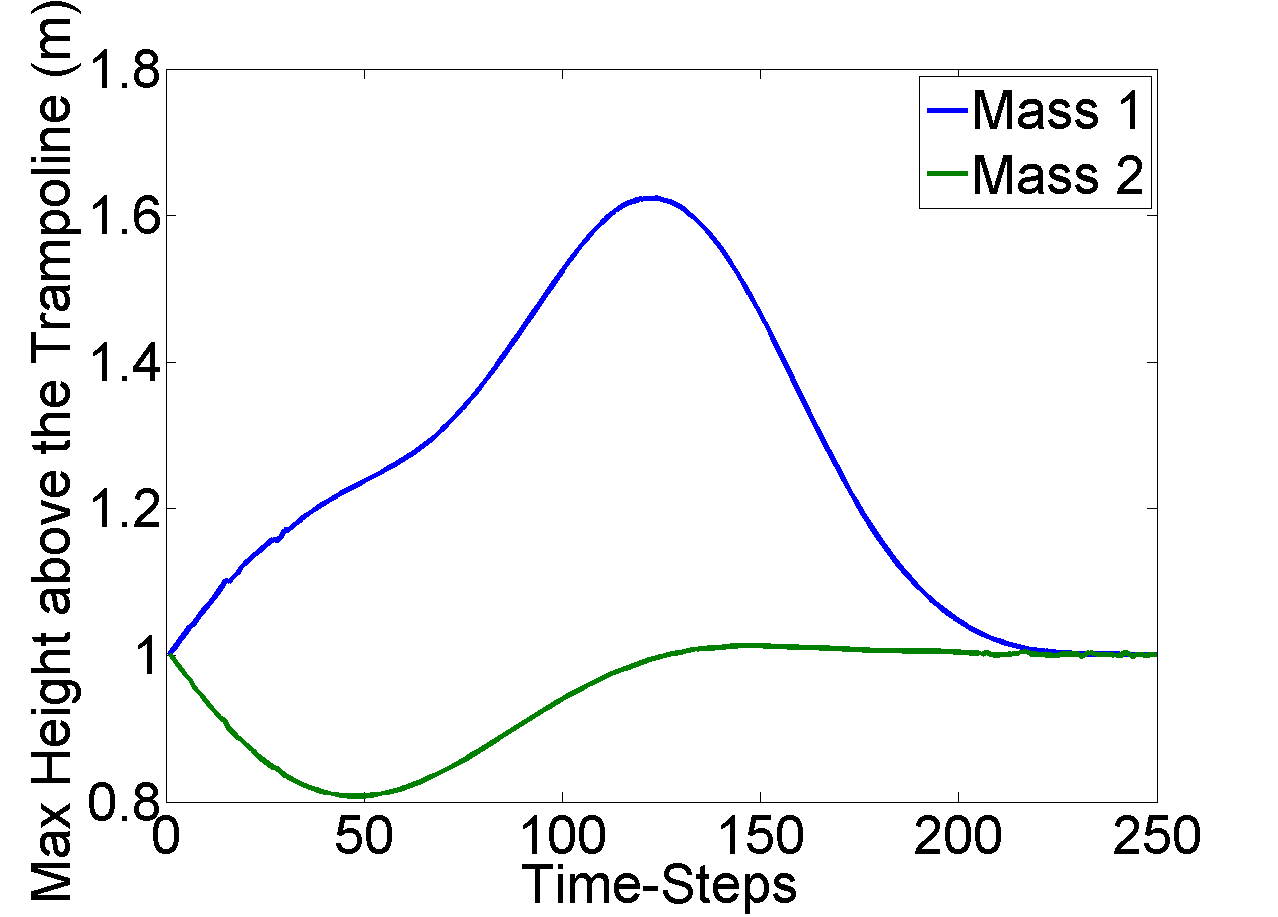
\includegraphics[width=\textwidth]{m1_on_tramp_same_masses_distance_14.png}
    	\caption{Maximum heights reached when $m_1$ and $m_2$ are the same mass and $m_1$ starts on the trampoline.}\label{fig:m1_on_tramp_same_masses_distance_14}
    \end{subfigure}\hfill
    \caption{The maximum heights reached by $m_1$ and $m_2$ for a range of time-steps. The distance between the masses is kept constant at 1.4m.}\label{fig:distance_14}
\end{figure}

%mass one (lighter) on tramp then mass two (heavier) dropped
\noindent As can be seen from Figure \ref{fig:m1_on_tramp_different_masses_distance_14}, when the time step is at 0, meaning that both masses hit the trampoline at the same time, they reach close to their starting heights. As the time step increases to 50 (and mass two is hitting the trampoline after mass one), there is a swap of which mass travels to the greatest height. Then, as the time step increases around 125, the height of mass ones bounce is around double the height of mass two's, showing that there is a transfer of energy. As the time step increases to around 190, there is another swap in the maximum heights, and mass two begins to travel higher than mass one again. Then, as the time step increases to 250, the masses begin to travel to about their starting heights only. \\

%mass one (lighter) dropped then mass two (heavier) on tramp

\noindent In Figure \ref{fig:m2_on_tramp_different_masses_distance_14}, mass two, the heavier mass, is on the trampoline and mass one is dropped on to the trampoline. At time step 0, both masses once again reach their starting height. As the time step increases to 100, mass one begins to reach a higher height than it's starting height (around 1.85m) and mass two reaches a slightly lower height (about 1.32m). This shows a very small transfer of energy between the two masses. As the time step continues to increase to 250, the masses return to travelling to their starting heights. \\
%mass one (equal) on tramp and mass two (equal) dropped

\noindent Figure \ref{fig:m1_on_tramp_same_masses_distance_14} shows equal masses one and two hitting the trampoline. When the time step is 0, they travel to the same height, as is expected. As the time step increases however, and mass two hits the trampoline after mass one, mass one gets a maximum height increase, and mass two has a height decrease, until the time step reaches 100 and mass two  reaches its starting height. At this point, the maximum height of mass one begins the decrease and converges to the height of mass two again at around 225.



%include diagram drawings of the systems.

\subsection{Modelling Various Distances Between the Masses}\label{res2}
\noindent Taking a cut-through of the three dimensional graphs in Figures \ref{fig:m1on3d}, \ref{fig:m2on3d} and \ref{fig:msameon3d} for a consistently selected time-step can now compare the relationship between varying distance and height between the two masses for a multitude of positions. The time-step chosen is 125, the point where displacement is lowest. 

\begin{figure}[H]
	\centering
    \begin{subfigure}[t]{0.3\textwidth}
		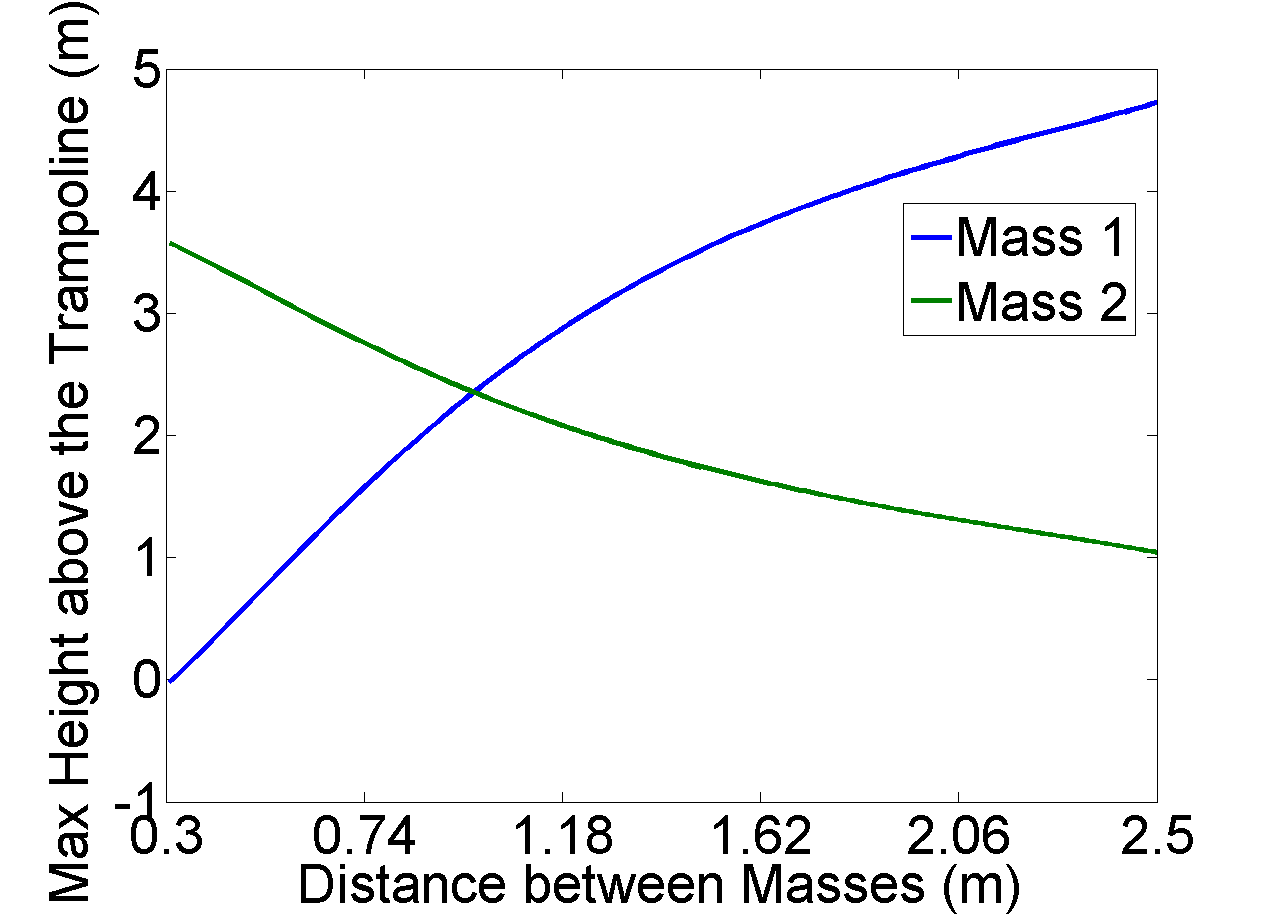
\includegraphics[width=\textwidth]{m1_on_tramp_different_masses_timestep_125.png}
    	\caption{Maximum heights reached when $m_1$ and $m_2$ are different masses and $m_1$ starts on the trampoline.}\label{fig:m1_on_tramp_different_masses_timestep_125}
    \end{subfigure}\hfill
	\begin{subfigure}[t]{0.3\textwidth}
		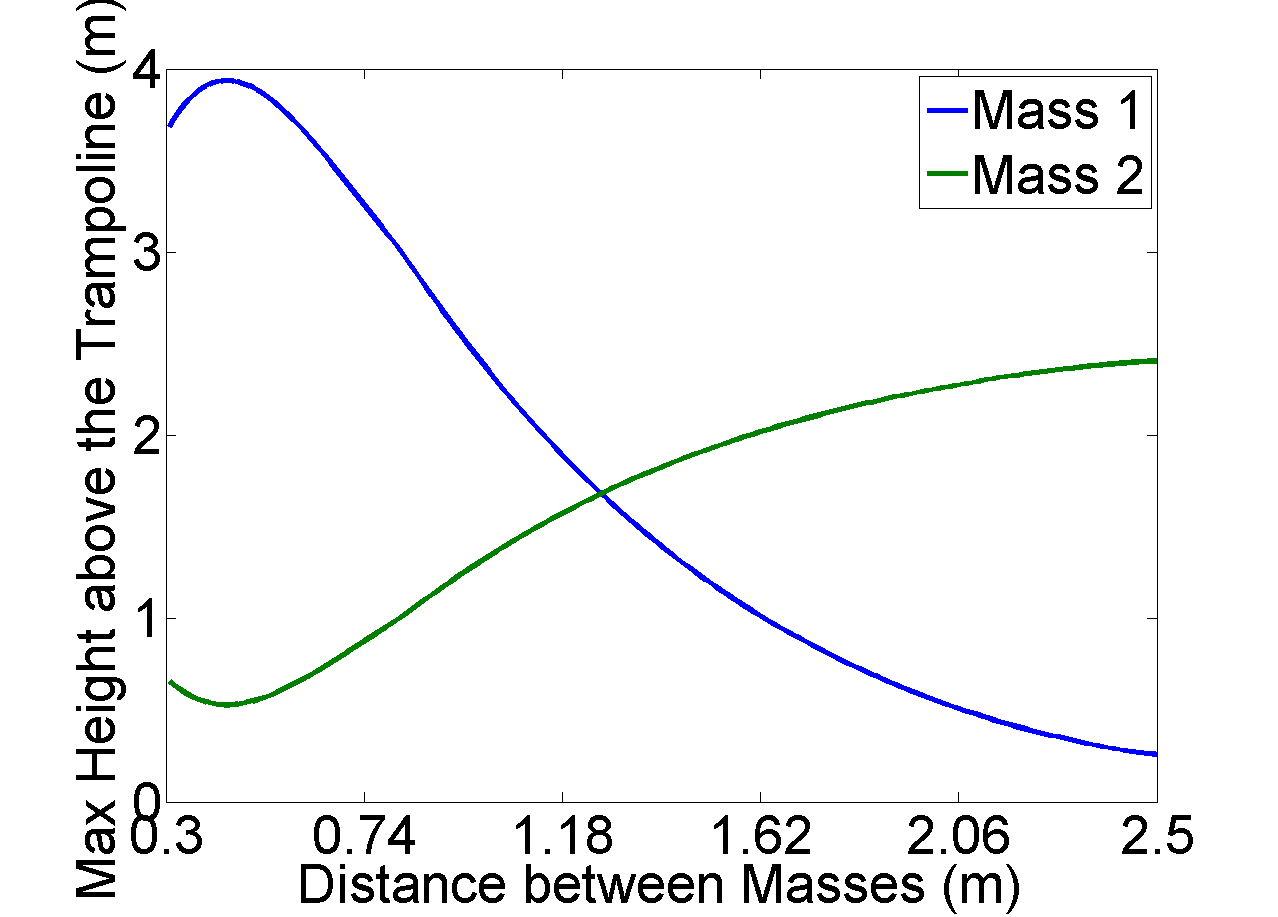
\includegraphics[width=\textwidth]{m2_on_tramp_different_masses_timestep_125.png}
    	\caption{Maximum heights reached when $m_1$ and $m_2$ are different masses and $m_2$ starts on the trampoline.}\label{fig:m2_on_tramp_different_masses_timestep_125}
    \end{subfigure}\hfill
    \begin{subfigure}[t]{0.3\textwidth}
		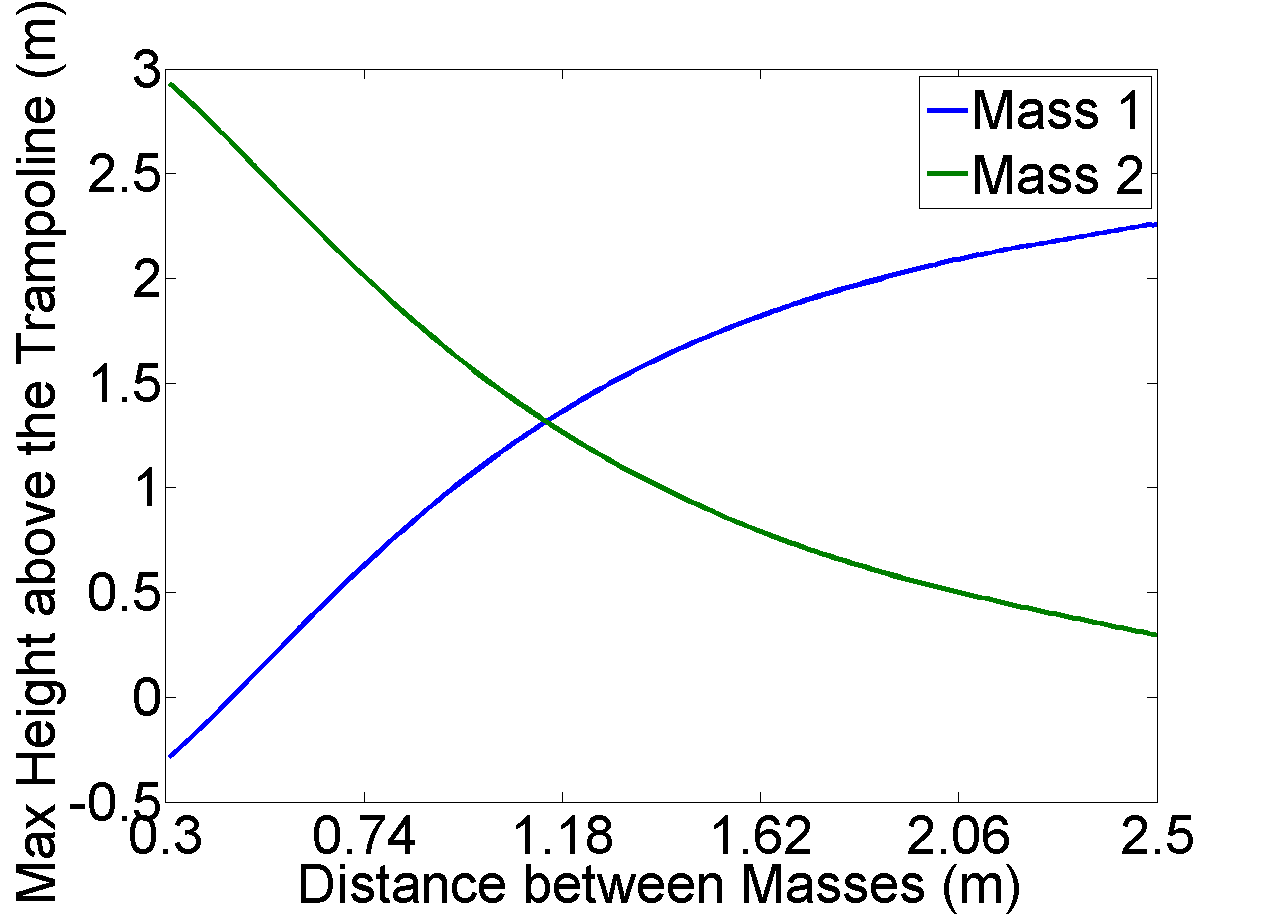
\includegraphics[width=\textwidth]{m1_on_tramp_same_masses_timestep_125.png}
    	\caption{Maximum heights reached when $m_1$ and $m_2$ are the same masses and $m_1$ starts on the trampoline.}\label{fig:m1_on_tramp_same_masses_timestep_125}
    \end{subfigure}\hfill
    \caption{The maximum heights reached by $m_1$ and $m_2$ for a range of distances between the two masses. The time-step is kept constant at 125.}\label{fig:timestep_125}
\end{figure}

\noindent For the case where the lighter mass, mass one, is dropped first the behaviour of the system is seen in Figure \ref{fig:m1_on_tramp_different_masses_timestep_125}. The graph shows that as the distance between masses increases, the maximum height reached by mass one increases and decreases for mass two. The rate at which mass one's maximum height increases is faster than the rate at which mass two's decreases. The mass reaching greatest height swaps at a small distance between from mass two and one. %similar/different to equal masses?
\\
\\
\noindent Figure \ref{fig:m2_on_tramp_different_masses_timestep_125} shows the system set up with the heavier mass, mass two, dropped first. The maximum height of mass one reached increases slightly before decreasing as distance between masses increases. The maximum height of mass two decreases slightly before increasing as distance between masses increases. Mass one maximum height varies far more than mass. The mass reaching greatest height swaps at larger distance between mass one and two than seen in \ref{fig:m1_on_tramp_different_masses_timestep_125} metres apart from mass one and two.  \\
\\
\noindent When considering two masses of equal mass, chosen as 50 kg, the results are shown in \ref{fig:m1_on_tramp_same_masses_timestep_125}. The graph shows very similar behaviour to Figure \ref{fig:m1_on_tramp_different_masses_timestep_125}, with lower maximum heights reached for mass one and higher maximum heights for mass two. The mass reaching greatest height swaps at a low distance between mass two and one. 

\subsection{Finding Optimal Time-Steps and Distances between Masses}

\noindent Taking a top-down view of Figures \ref{fig:m1on3d}, \ref{fig:m2on3d} and \ref{fig:msameon3d} in Section \ref{3d} and using the colour map gives an output where the maximum heights for all combinations of position and time lag can be visualised for both masses. Figures \ref{fig:m1upm1on} shows that mass one reaches heights approaching 5 metres for the cases when the two masses are placed far apart and the time-step is approximately at the halfway interval. This means, with reference to Figure \ref{fig:dvt}, that mass one is currently near its most negative value for y displacement.
Simultaneously, as shown by Figure \ref{fig:m2upm1on} mass two does not reach large heights in these instances, as expected. 
\noindent Figure \ref{fig:m1upm2on} shows the case where mass two is in contact with the trampoline before mass one.  Figure \ref{fig:m2upm2on} follows the same height distribution as seen in Figure \ref{fig:m1upm1on} as the same behaviour of masses is observed, i.e. the first mass in contact with the trampoline is the first to leave, with a greater height.  Due to mass two being heavier, it does not reach a height as great as mass one. Comparing Figures \ref{fig:m2upm1on} and \ref{fig:m1upm2on} again shows similar behaviour.

\begin{figure}[H]
	\centering
    \begin{subfigure}{0.45\textwidth}
		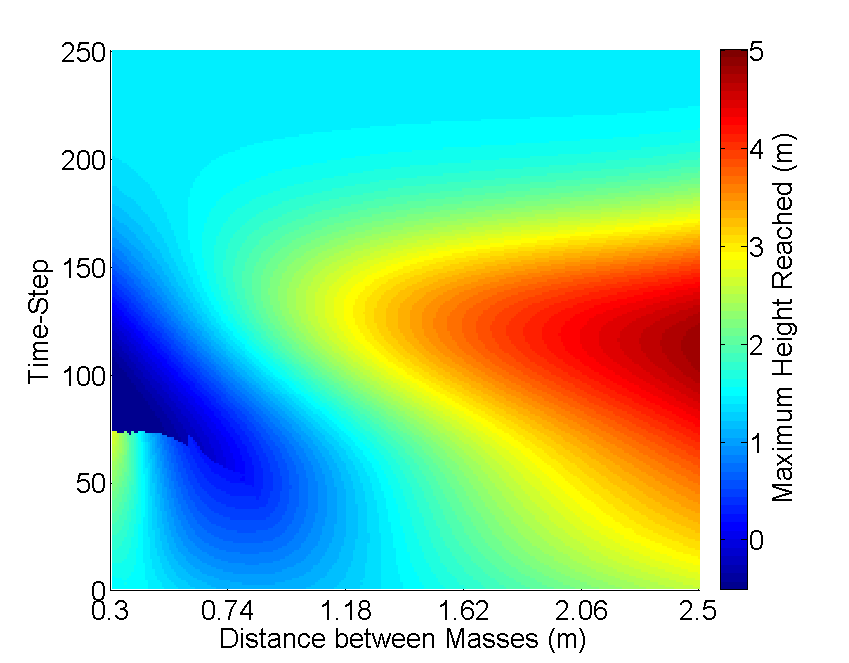
\includegraphics[width=3.1in, height=2in]{Hm1on_m1.png}
    	\caption{The maximum height of mass one.}\label{fig:m1upm1on}
    \end{subfigure}\hfill
	\begin{subfigure}{0.45\textwidth}
		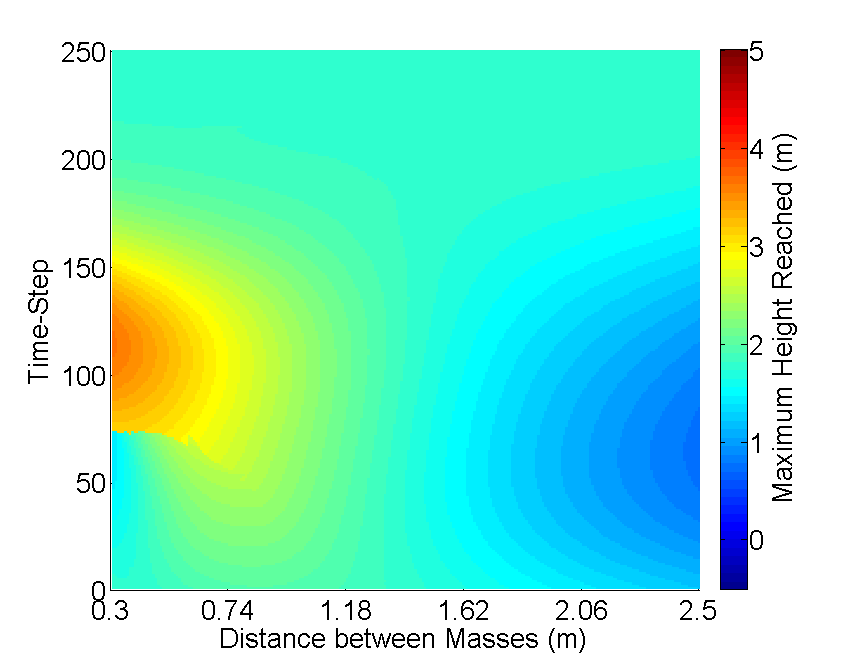
\includegraphics[width=3.1in, height=2in]{Hm1on_m2.png}
    	\caption{The maximum height of mass two.}\label{fig:m2upm1on}
    \end{subfigure}\hfill
    \begin{subfigure}{0.45\textwidth}
		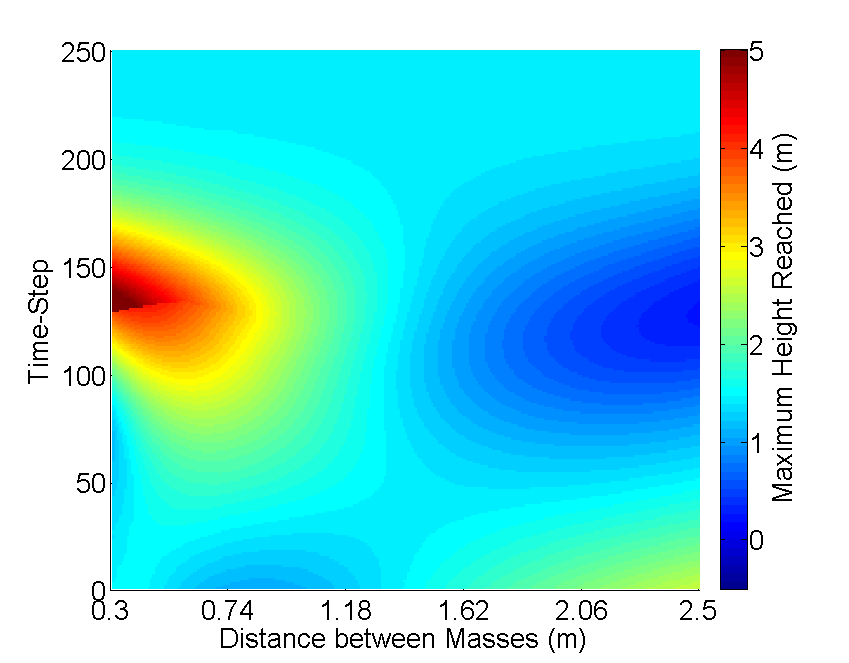
\includegraphics[width=3.1in, height=2in]{Hm2on_m1.png}
    	\caption{The maximum height of mass one.}\label{fig:m1upm2on}
    \end{subfigure}\hfill
	\begin{subfigure}{0.45\textwidth}
		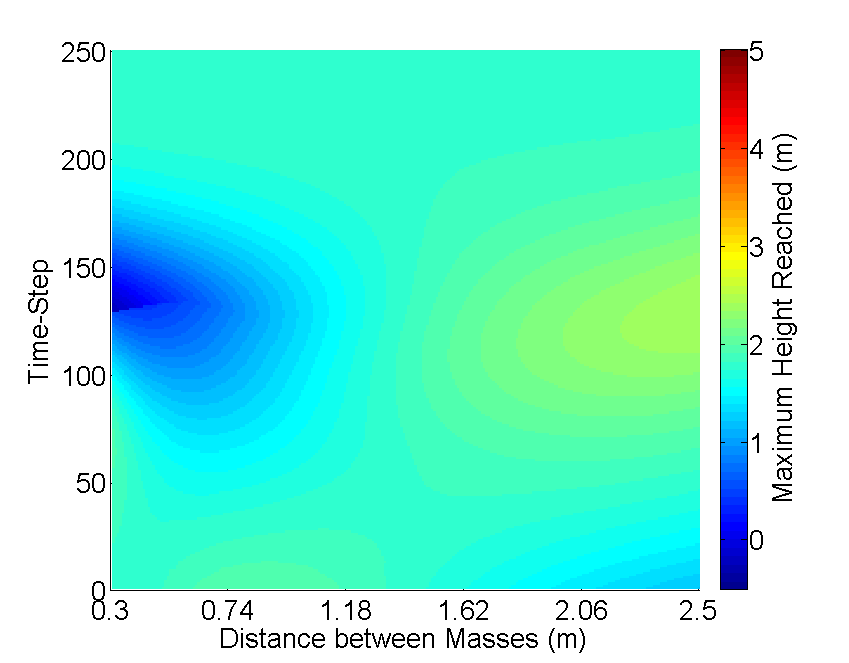
\includegraphics[width=3.1in, height=2in]{Hm2on_m2.png}
    	\caption{The maximum height of mass two.}\label{fig:m2upm2on}
    \end{subfigure}\hfill
    \caption{Surface plots showing the maximum heights reached by each mass given a range of distances between them, and during different time-steps. $m_1$ has a starting height of 1.44m and $m_2$ has a starting height of 1.8m. Figures \ref{fig:m1upm1on} and \ref{fig:m2upm1on} show the results when $m_1$ was on the trampoline first. Figures \ref{fig:m1upm2on} and \ref{fig:m2upm2on} show the same test when $m_2$ was on the trampoline first.}\label{fig:mup1on}
\end{figure}


\noindent Figure \ref{fig:msup} shows the same interactions between the masses when they are of an equal mass of 50kg, as described in Section \ref{vid}. Mass one comes into contact with the trampoline first in this test and is the one to leave with greatest energy, as before. Figure \ref{fig:m2sup} shows that it does not reach as great heights as seen in \ref{fig:m1upm1on}, when the smaller mass leaves the trampoline, but does have a greater maximum height than in the case where the greater mass leaves the trampoline, seen in Figure \ref{fig:m2upm2on}. This makes sense because a mass gains more energy from an equal mass than one with a lesser amount. Figure \ref{fig:m1sup} fits this same in-between levels of intensity on the contour map.
\begin{figure}[H]
	\centering
    \begin{subfigure}{0.45\textwidth}
		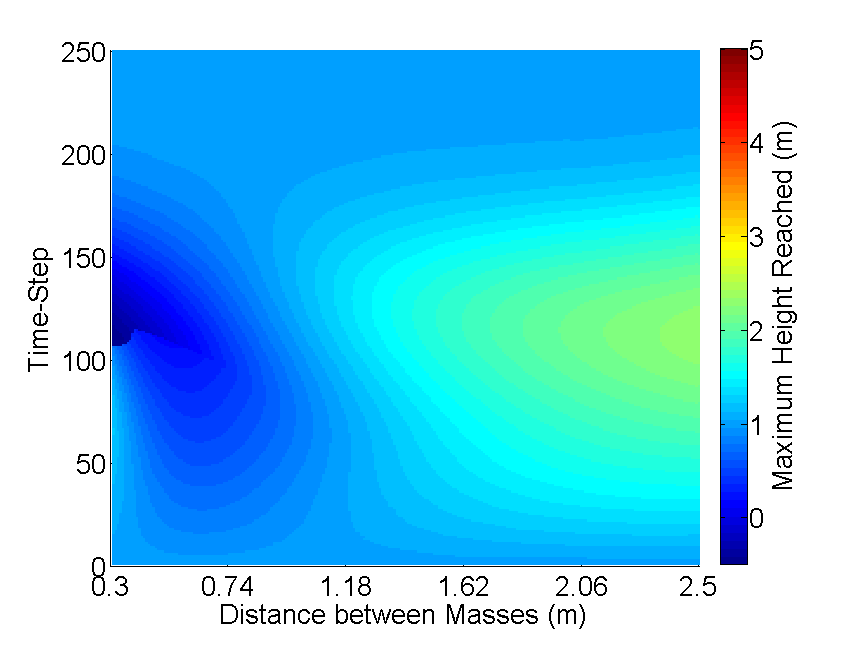
\includegraphics[width=3.1in, height=2in]{Hmson_m2.png}
    	\caption{The maximum height of mass one.}\label{fig:m1sup}
    \end{subfigure}\hfill
	\begin{subfigure}{0.45\textwidth}
		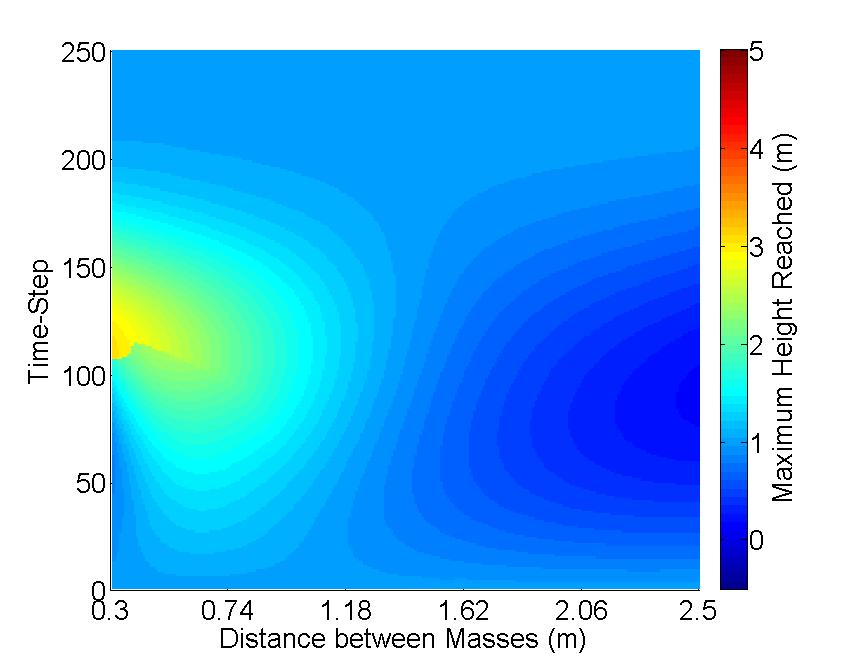
\includegraphics[width=3.1in, height=2in]{Hmson_m1.png}
    	\caption{The maximum height of mass two.}\label{fig:m2sup}
    \end{subfigure}\hfill
    \caption{Surface plots showing the maximum height when the added mass is placed at different lengths away from the other mass at different times.}\label{fig:msup}
\end{figure}




\subsection{Points of Interest}

\begin{figure}[H]
	\centering
	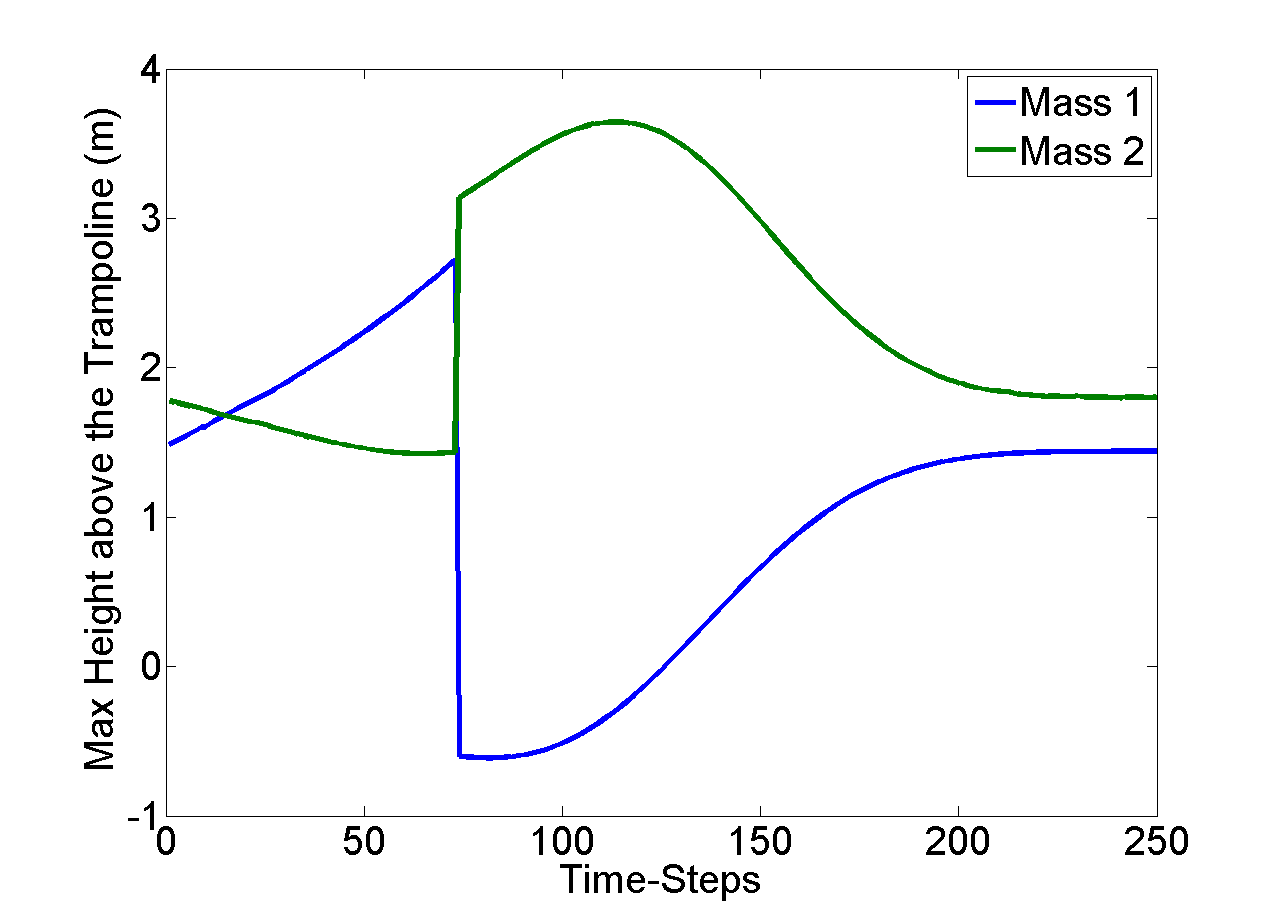
\includegraphics[width=3.1in, height=2in]{points_of_interest.png}
    \caption{A graph showing the maximum heights of both masses when $m_1$ and $m_2$ are different masses and $m_1$ starts on the trampoline. The two masses are 0.3m apart.}\label{fig:poi}
\end{figure}

\noindent By studying the 3D graphs, it was clear that there were a few other points of interest. For example, when the distance between the masses is small there is a sharp change in maximum heights of the masses at a certain time-step. This is illustrated, at a time step of 70, in Figure \ref{fig:poi}. At this time step, $m_2$ becomes the mass which is jumping higher, whereas before it was $m_1$. This is happening because, before the $70^{th}$ time-step $m_1$ is the first mass to leave the trampoline and after the time-step, $m_2$ is first mass to leave the trampoline. This suggests that the first mass to leave the trampoline will always be the mass which travels the highest. \\

\noindent Another point of interest seen in Figure \ref{fig:poi} is that, for a short time after the $70^{th}$ time step, the maximum height of $m_1$ is negative. This means that the mass does not travel above the starting height of the trampoline when it leaves. The reason for this is that there is a complete transfer of kinetic energy between the two masses, meaning $m_1$ has very little velocity when it leaves the trampoline.


%%%%%%%%% further away higher jump - seen in all cases where heavy mass on first, light mass on first and where both masses weigh the same.


